The Standard Model is a very well tested theory capable of giving precise
predictions on particles and their interactions. \cref{fig:sm_summary_plot}
gives the comparison between experimental measurements performed by the
\gls{atlas} collaboration and theoretical predictions for several Standard Model
production cross sections, in general the predictions agree with the measured
data. \cref{fig:higgs_summary_plot} reports the measured signal strength for a
Higgs boson mass of 125.36~GeV normalized to the Standard Model expectations in
H$\rightarrow \gamma \gamma$,
H$\rightarrow ZZ^* \rightarrow \ell \ell \ell \ell$,
H$\rightarrow W W^* \rightarrow \ell \nu \ell \nu$, H$\rightarrow \tau \tau$ and
H$\rightarrow b \bar{b}$ final states, as can be seen the \gls{atlas}
collaboration has, within uncertainties, sensitivity in most of these searches.
\begin{figure}[!h]
  \centering
  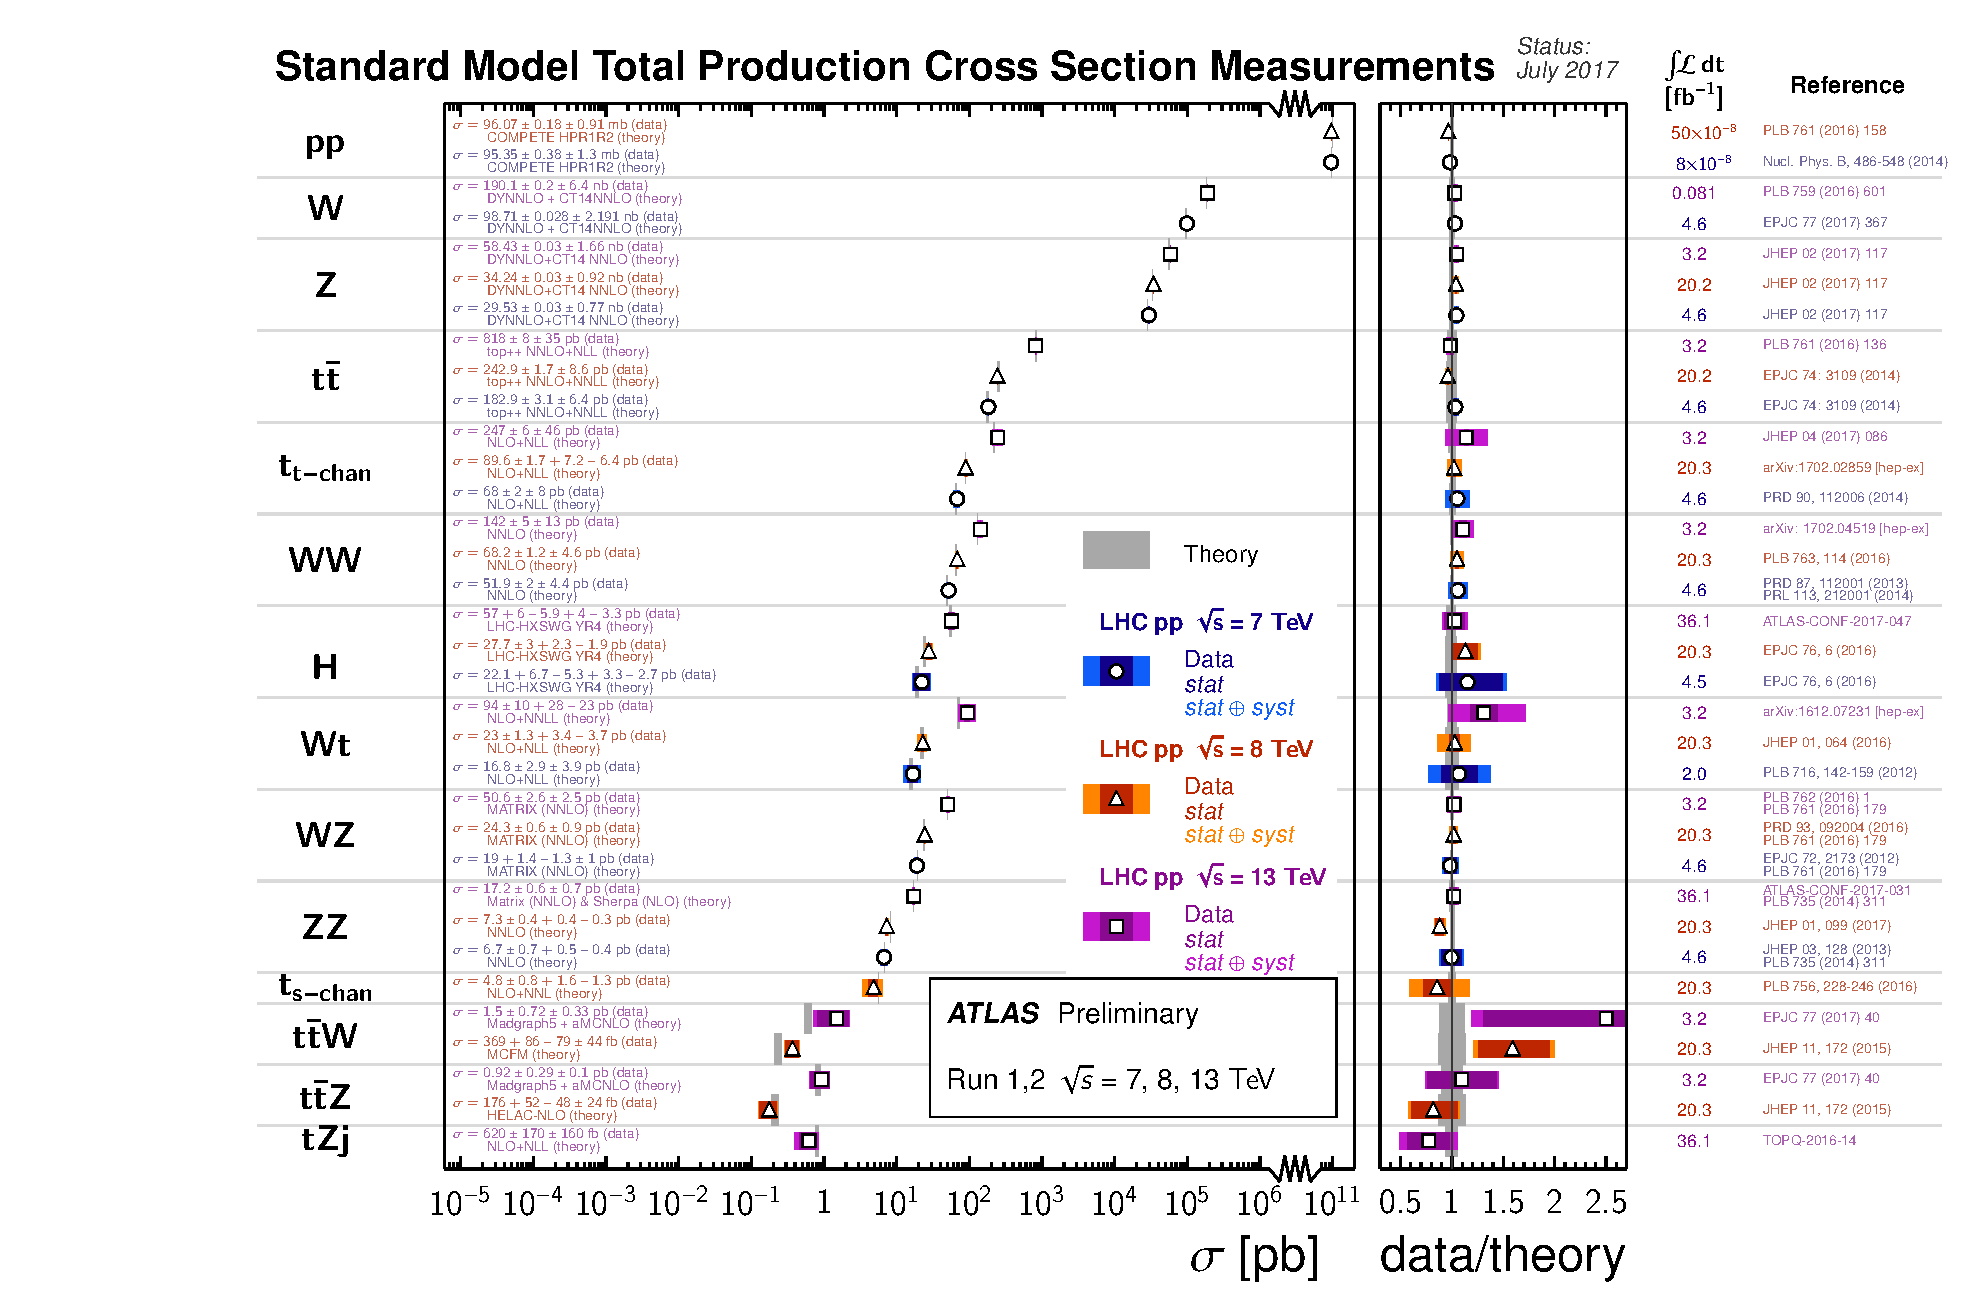
\includegraphics[width=\linewidth]{atlas_sm_summary}
  \caption{Comparison between experimental measurements and theoretical
    predictions for several Standard Model production cross sections corrected
    for leptonic branching fractions. The statistical uncertainty is reported in
    the plot with a dark-colored error bar. The light-colored error band
    represents the full uncertainty including statistics, systematics and
    luminosity uncertainties. The reference for each measurement as long as the
    ratio between data and theoretical prediction are also reported in the
    plot~\cite{SMPubPlots}.}
  \label{fig:sm_summary_plot}
\end{figure}
\begin{figure}[!h]
  \centering
  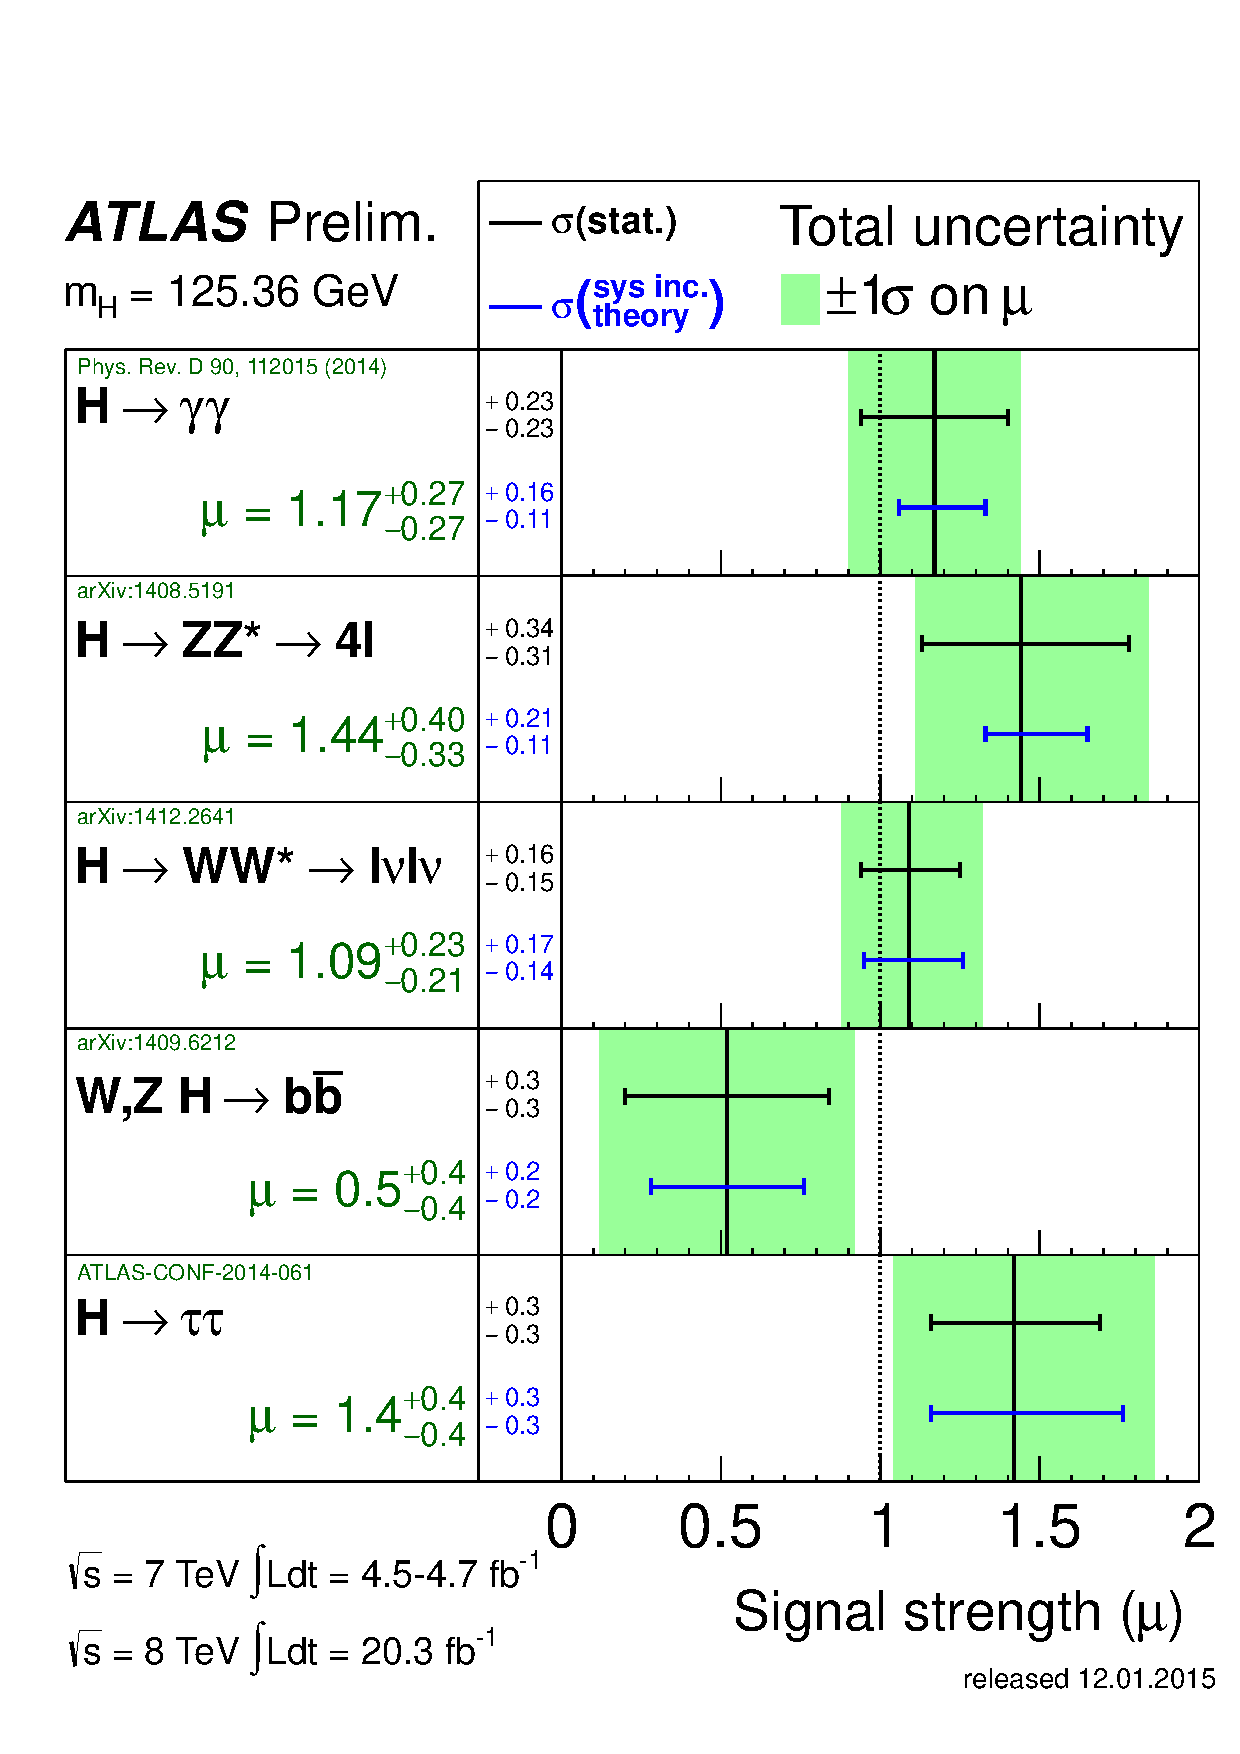
\includegraphics[scale=.5]{atlas_higgs_summary}
  \caption{Measured signal strength for a Higgs boson mass of 125.36~GeV
    normalized to the Standard Model expectations in
    H$\rightarrow \gamma \gamma$,
    H$\rightarrow ZZ^* \rightarrow \ell \ell \ell \ell$,
    H$\rightarrow W W^* \rightarrow \ell \nu \ell \nu$, H$\rightarrow \tau \tau$
    and H$\rightarrow b \bar{b}$ final states. The solid vertical lines
    represent the best fitted value, the shaded band is the total $\pm 1 \sigma$
    uncertainty. The statistical and total (experimental and theoretical)
    individual uncertainties are also reported~\cite{HiggsPubPlots}.}
  \label{fig:higgs_summary_plot}
\end{figure}
%%% Local Variables:
%%% mode: latex
%%% TeX-master: "../search_for_DM_LED_with_ATLAS"
%%% End:
